The conduction heat transfer is described by Equation \ref{condu}:
\begin{equation}
\rho c_{P}\frac{\partial T}{\partial t}=\nabla\cdot\left(\lambda\nabla T\right)+\dot{q}_{v}
\label{condu}
\end{equation}
Where $\rho$ is the density, T the temperature, $\lambda$ the conductivity of the material, $c_{P}$ the specific heat of the material and $\dot{q}_{v}$ the inner heat of the material (source term).

\section{Four materials}
The four materials problem is a two-dimensional transient conduction problem. It consists in a long rod composed of four different materials with different properties. The general scheme of the problem is represented in figure \ref{fourmaterials}.
\begin{figure}[h]
	\centering
	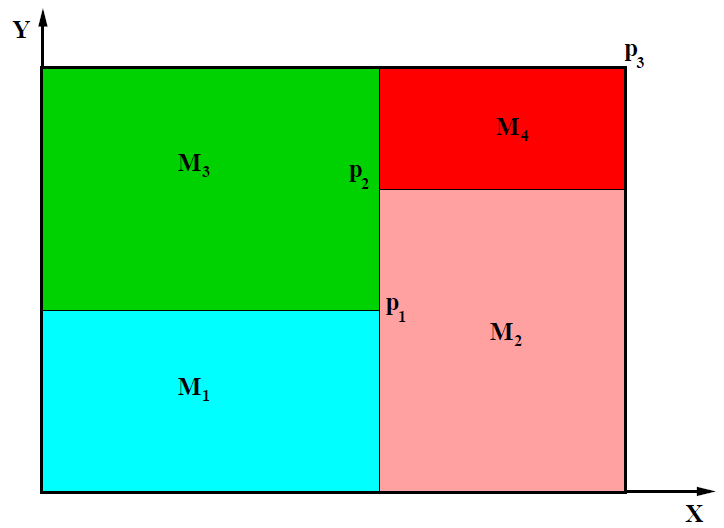
\includegraphics[scale = 0.8]{FourMaterials/Fourmaterials}
	\caption{General scheme of the four materials problem}
	\label{fourmaterials}
\end{figure}
\begin{table}[h!]
	\centering
	\begin{tabular}{ |c|c|c|}
		\hline
		  & x [m] & y [m] \\ \hline
		 $p_{1}$ & $0.50$ & $0.40$ \\ \hline
		 $p_{2}$ & $0.50$ & $0.70$ \\ \hline
		 $p_{3}$ & $1.10$ & $0.80$ \\ \hline
	\end{tabular}
\caption{Problem coordinates}
\end{table}
\begin{table}[h!]
	\centering
	\begin{tabular}{ |c|c|c|c| }
		\hline
		& $\rho [kg/m^{3}]$ & $c_{P} [J/kgK]$ & $\lambda [W/mK]$ \\ \hline
		$M_{1}$ & $1500.00$ & $750.00$ & $170.00$ \\ \hline
		$M_{2}$ & $1600.00$ & $770.00$ & $140.00$ \\ \hline
		$M_{3}$ & $1900.00$ & $810.00$ & $200.00$ \\ \hline
		$M_{4}$ & $2500.00$ & $930.00$ & $140.00$ \\ \hline
	\end{tabular}
\caption{Physical properties of the materials}
\end{table}
\begin{table}
	\centering
	\begin{tabular}{ |c|c|}
		\hline
		Cavity wall & Boundary condition \\ \hline
		Bottom & Isotherm at $T=23.00 ºC$ \\ \hline
		Top & Uniform $Q_{flow}=60.00 W/m$ length \\ \hline
		Left & In contact with a fluid at $T_{g}=33.00 ºC$ and heat transfer coefficient $9.00 W/m^{2}K$ \\ \hline
		Right & Uniform temperature $T=8.00+0.005t ºC$ (where $t$ is the time in seconds) \\ \hline
	\end{tabular}
\caption{Boundary conditions}
\end{table}

The initial temperature field is $T=8.00 ºC$.

\section{Discretization}
The domain is discretized using the node centred distribution, to avoid having conflictive control volumes between the different materials. Since it is a transitory problem, it is necessary to discretize in space and time. The method used to discretize the equation is the finite volume method.

\subsection{Spatial discretization}
\begin{figure}
	\centering
	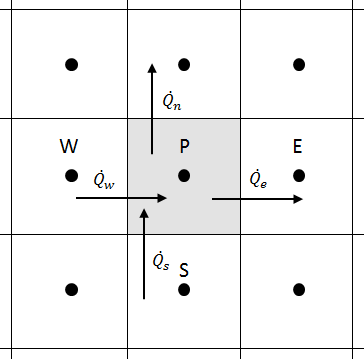
\includegraphics[]{FourMaterials/controlvolume2d}
	\caption{Heat fluxes through the faces of a control volume}
	\label{convol2d}
\end{figure}
The heat fluxes through the walls represented in figure \ref{convol2d} are integrated:
\begin{equation}
\dot{Q}_{e}=-\int_{}^{S_{e}}\lambda\frac{\partial T}{\partial x}dS\approx-\left(\lambda\frac{\partial T}{\partial x}\right)_{e}S_{e}\approx-\lambda_{e}\frac{T_{E}-T_{P}}{d_{PE}}S_{e}
\end{equation}
\begin{equation}
\dot{Q}_{w}=-\int_{}^{S_{w}}\lambda\frac{\partial T}{\partial x}dS\approx-\left(\lambda\frac{\partial T}{\partial x}\right)_{w}S_{w}\approx-\lambda_{w}\frac{T_{P}-T_{W}}{d_{PW}}S_{w}
\end{equation}
\begin{equation}
\dot{Q}_{n}=-\int_{}^{S_{n}}\lambda\frac{\partial T}{\partial x}dS\approx-\left(\lambda\frac{\partial T}{\partial x}\right)_{n}S_{n}\approx-\lambda_{n}\frac{T_{N}-T_{P}}{d_{PN}}S_{n}
\end{equation}
\begin{equation}
\dot{Q}_{s}=-\int_{}^{S_{s}}\lambda\frac{\partial T}{\partial x}dS\approx-\left(\lambda\frac{\partial T}{\partial x}\right)_{s}S_{s}\approx-\lambda_{s}\frac{T_{P}-T_{S}}{d_{PS}}S_{s}
\end{equation}
where $T$ is the temperature at the given node, $d$ the distance between two nodes, and $\lambda$ the conductivity at the given face.
However, since there are different materials there are faces in which the conductivity can have two values: one on the left side of the face and the other one on the right side of the face. This problem is solved with the harmonic mean. It can be calculated with the heat fluxes through the wall:
\begin{equation*}
\dot{q}_{e}^{-}=\dot{q}_{e}^{+}
\end{equation*}
\begin{equation*}
-\lambda_{P}\frac{T_{e}-T_{P}}{d_{Pe}}=-lambda_{E}\frac{T_{E}-T_{e}}{d_{Ee}}
\end{equation*}
\begin{equation*}
	\dot{q}_{e}=-lambda_{e}\frac{T_{E}-T_{P}}{d_{PE}}
\end{equation*}
\begin{equation}
\lambda_{e}=\frac{d_{PE}}{\frac{d_{Pe}}{\lambda_{P}}+\frac{d_{Ee}}{\lambda_{E}}}
\end{equation}
The inner heat of the material can be discretized as:
\begin{equation}
Q_{VP}=\int_{V_{P}}^{}\dot{q}_{v}dV\approx\dot{q}_{vP}V_{P}
\end{equation}

\subsection{Time discretization}
The time discretization is done using the First law of thermodynamics:
\begin{equation}
\int_{V_{P}}^{}\rho\frac{\partial u}{\partial t}dV=\sum\dot{Q}_{P}
\end{equation}
where $u$ is the internal energy of the control volume.
Assuming an incompressible material, the First law of thermodynamics is integrated over time. Taking $n$ as the previous instant of time and $n+1$ the instant of time that is going to be calculated:
\begin{equation}
\int_{t^{n}}^{t^{n+1}}\rho_{P}\frac{\partial\bar{u}_{P}}{\partial t}V_{P}dt=\int_{t^{n}}^{t^{n+1}}\sum\dot{Q}_{P}dt
\end{equation}
Rearranging the first term of the equation:
\begin{equation*}
\int_{t^{n}}^{t^{n+1}}\rho_{P}\frac{\partial\bar{u}_{P}}{\partial t}V_{P}dt=\rho_{P}V_{P}\left(\bar{u}_{P}^{n+1}-\bar{u}_{P}^{n}\right)\approx\rho_{P}V_{P}\left(u_{P}^{n+1}-u_{P}^{n}\right)=\rho_{P}V_{P}\bar{c}_{P}\left(T_{P}^{n+1}-T_{P}^{n}\right)
\end{equation*}
\begin{equation*}
	\int_{t^{n}}^{t^{n+1}}\sum\dot{Q}_{P}dt=\left[\beta\sum\dot{Q}_{P}^{n+1}+\left(1-\beta\right)\sum\dot{Q}_{P}^{n}\right]\Delta t
\end{equation*}
The discretized equation is finally obtained:
\begin{equation}
\rho_{P}V_{P}\bar{c}_{P}\frac{T_{P}^{n+1}-T_{P}^{n}}{\Delta t}=\beta\left[-\lambda_{w}\frac{T_{P}-T_{W}}{d_{PW}}S_{w}+\lambda_{e}\frac{T_{E}-T_{P}}{d_{PE}}S_{e}-\lambda_{s}\frac{T_{P}-T_{S}}{d_{PS}}S_{s}+\lambda_{n}\frac{T_{N}-T_{P}}{d_{PN}}S_{n}+\dot{q}_{vP}V_{P}\right]^{n+1}+\left(1-\beta\right)\left[-\lambda_{w}\frac{T_{P}-T_{W}}{d_{PW}}S_{w}+\lambda_{e}\frac{T_{E}-T_{P}}{d_{PE}}S_{e}-\lambda_{s}\frac{T_{P}-T_{S}}{d_{PS}}S_{s}+\lambda_{n}\frac{T_{N}-T_{P}}{d_{PN}}S_{n}+\dot{q}_{vP}V_{P}\right]^{n}
\end{equation}
To simplify the equation, it can be rewritten with coefficients, dependant on the properties of the nearest nodes in the following form:
\begin{equation}
a_{P}T_{P}=a_{E}T_{E}+a_{W}T_{W}+a_{N}T_{N}+a_{S}T_{S}+b_{P}
\end{equation}
The coefficients are called discretization coefficients, and they are different for each node. The discretization coefficients are:
\begin{equation}
a_{E}=\beta\frac{\lambda_{e}S_{e}}{d_{PE}}
\end{equation}
\begin{equation}
a_{W}=\beta\frac{\lambda_{w}S_{w}}{d_{PW}}
\end{equation}
\begin{equation}
a_{N}=\beta\frac{\lambda_{n}S_{n}}{d_{PN}}
\end{equation}
\begin{equation}
a_{S}=\beta\frac{\lambda_{s}S_{s}}{d_{PS}}
\end{equation}
\begin{equation}
a_{P}=a_{E}+a_{W}+a_{N}+a_{S}+\rho_{P}V_{P}\bar{c}_{P}/\Delta t
\end{equation}
\begin{equation}
b_{P}=\frac{\rho_{P}V_{P}\bar{c}_{P}T_{P}^{n}}{\Delta t}+\beta\dot{q}_{vP}^{n+1}V_{P}+\left(1-\beta\right)\left[-\lambda_{w}\frac{T_{P}-T_{W}}{d_{PW}}S_{w}+\lambda_{e}\frac{T_{E}-T_{P}}{d_{PE}}S_{e}-\lambda_{s}\frac{T_{P}-T_{S}}{d_{PS}}S_{s}+\lambda_{n}\frac{T_{N}-T_{P}}{d_{PN}}S_{n}+\dot{q}_{vP}V_{P}\right]^{n}
\end{equation}

\subsection{Boundary conditions}
The outer walls of the rod have special conditions, so each of them has to be studied in order to determine the coefficients of the boundary nodes.
In the left wall, there is convection, so some coefficients have to be recalculated:
\begin{equation}
a_{W}=0
\end{equation}
\begin{equation}
a_{P}=a_{E}+a_{W}+a_{N}+a_{S}+\frac{\rho_{P}V_{P}\bar{c}_{P}}{\Delta t}+\frac{\beta}{\frac{1}{\alpha}+\frac{d_{Pw}}{\lambda_{P}}}
\end{equation}
\begin{equation}
b_{P}=\frac{\rho_{P}V_{P}\bar{c}_{P}T_{P}^{n}}{\Delta t}+\beta\left(\dot{q}_{vP}^{n+1}V_{P}+\frac{T_{g}}{\frac{1}{\alpha}+\frac{d_{Pw}}{\lambda_{P}}}\right)+\left(1-\beta\right)\left[\frac{T_{g}-T_{P}}{\frac{1}{\alpha}+\frac{d_{Pw}}{\lambda_{P}}}+\lambda_{e}\frac{T_{E}-T_{P}}{d_{PE}}S_{e}-\lambda_{s}\frac{T_{P}-T_{S}}{d_{PS}}S_{s}+\lambda_{n}\frac{T_{N}-T_{P}}{d_{PN}}S_{n}+\dot{q}_{vP}V_{P}\right]^{n}
\end{equation}
In the top wall there is a constant heat flux. The new coefficients are:
\begin{equation}
a_{N}=0
\end{equation}
\begin{equation}
b_{P}=\frac{\rho_{P}V_{P}\bar{c}_{P}T_{P}^{n}}{\Delta t}+\beta\dot{q}_{vP}^{n+1}V_{P}+Q_{flow}\frac{S_{n}}{S_{top}}+\left(1-\beta\right)\left[-\lambda_{w}\frac{T_{P}-T_{W}}{d_{PW}}S_{w}+\lambda_{e}\frac{T_{E}-T_{P}}{d_{PE}}S_{e}-\lambda_{s}\frac{T_{P}-T_{S}}{d_{PS}}S_{s}+\dot{q}_{vP}V_{P}\right]^{n}
\end{equation}
In the right wall, the temperature $T_{r}$ is given, and it changes over time. The coefficients are very similar to those of the general case. The only differences are:
\begin{equation}
a_{E}=0
\end{equation}
\begin{equation}
a_P=a_{E}+a_{W}+a_{N}+a_{S}+\frac{\rho_{P}V_{P}\bar{c}_{P}}{\Delta t}+\beta\frac{\lambda_{P}S_{e}}{d_{Pe}}
\end{equation}
\begin{equation}
b_{P}=\frac{\rho_{P}V_{P}\bar{c}_{P}T_{P}^{n}}{\Delta t}+\beta\left(\dot{q}_{vP}^{n+1}V_{P}+\frac{\lambda_{P}S_{e}}{d_{Pe}}T_{r}^{n+1}\right)+\left(1-\beta\right)\left[-\lambda_{w}\frac{T_{P}-T_{W}}{d_{PW}}S_{w}+\lambda_{P}\frac{T_{r}-T_{P}}{d_{Pe}}S_{e}-\lambda_{s}\frac{T_{P}-T_{S}}{d_{PS}}S_{s}+\lambda_{n}\frac{T_{N}-T_{P}}{d_{PN}}S_{n}+\dot{q}_{vP}V_{P}\right]^{n}
\end{equation}
Finally, in the bottom the temperature $T_{b}$ is also given, but it is constant. The approach is very similar to that of the right wall. So that the coefficients are:
\begin{equation}
a_{S}=0
\end{equation}
\begin{equation}
a_P=a_{E}+a_{W}+a_{N}+a_{S}+\frac{\rho_{P}V_{P}\bar{c}_{P}}{\Delta t}+\beta\frac{\lambda_{P}S_{s}}{d_{Ps}}
\end{equation}
\begin{equation}
b_{P}=\frac{\rho_{P}V_{P}\bar{c}_{P}T_{P}^{n}}{\Delta t}+\beta\left(\dot{q}_{vP}^{n+1}V_{P}+\frac{\lambda_{P}S_{s}}{d_{Ps}}T_{b}\right)+\left(1-\beta\right)\left[-\lambda_{w}\frac{T_{P}-T_{W}}{d_{PW}}S_{w}+\lambda_{e}\frac{T_{E}-T_{P}}{d_{PE}}S_{e}-\lambda_{P}\frac{T_{P}-T_{b}}{d_{Ps}}S_{s}+\lambda_{n}\frac{T_{N}-T_{P}}{d_{PN}}S_{n}+\dot{q}_{vP}V_{P}\right]^{n}
\end{equation}